\documentclass[journal]{IEEEtran}

\usepackage{tabularx}
\usepackage{amsmath}
\usepackage{graphicx}
%\usepackage{caption}  %centers the captions
\usepackage{float}
\usepackage[strings]{underscore}
\usepackage{cite}
\usepackage{url}
\usepackage{hyperref}
\usepackage{pdfpages}
\hypersetup{
    bookmarks=true,         % show bookmarks bar?
    unicode=false,          % non-Latin characters in Acrobat’s bookmarks
    pdftoolbar=true,        % show Acrobat’s toolbar?
    pdfmenubar=true,        % show Acrobat’s menu?
    pdffitwindow=true, %false,     % window fit to page when opened
    pdfstartview={FitH},    % fits the width of the page to the window
    pdftitle={Stock Market Prediction Using a Voting Machine Learning Model for Dow Jones Industrial Average Companies},    % title
    pdfauthor={Barry Wu},     % author
    pdfsubject={Stock Market Prediction},   % subject of the document
    pdfcreator={Barry Wu},   % creator of the document
    pdfproducer={Barry Wu}, % producer of the document
    pdfkeywords={Machine Intelligence, Machine Learning, Support Vector Machine, SVM, Ridge Regression, Elastic Regression, Bagged Tree, Random Forest, Ada Boost, Gradient Boost, General Boost, Stock Market Prediction}, % list of keywords
    pdfnewwindow=true,      % links in new PDF window
    colorlinks=true,%false,       % false: boxed links; true: colored links
    linkcolor=black, %red,          % color of internal links (change box color with linkbordercolor)
    citecolor=black,%green,        % color of links to bibliography
    filecolor=black,%magenta,      % color of file links
    urlcolor=blue,%cyan           % color of external links
}

\begin{document}
%%%%%%%%%%% Title
\title{Stock Market Prediction Using a Voting Machine Learning Model for Dow Jones Industrial Average Companies}

%%%%%%%%%%% Top left header
\markboth{CMPE-667 Machine Intelligence Term Project, December 2018}
{CMPE-667 Machine Intelligence Term Project, December 2018}

%%%%%%%%%%% Author
\author{\thanks{\hrulefill}Barry Wu$^{1}$\thanks{$^{2}$Barry Wu is a 5$^{th}$ year student from the Computer Engineering Department in Rochester Institute of Technology, Rochester, NY 14623, USA. (email: \href{mailto:bxw8904@rit.edu}{bxw8904@rit.edu})}}

\maketitle

%%%%%%%%%%% Abstract
\begin{abstract}
Investments into the stock market can either make one a powerful elite in a nation or a person with no value. This gamble for wealth is unpredictable as the stock market is highly volatile. Those who succeed in the stock market will be glorified for their fame and fortune. Examples of these people include Warren Buffet (CEO of Berkshire Hathaway) and Winklevoss Twins (investors of Bitcoins). Although many try to emulate these investor’s investment strategies, some have begun using machine learning models to help make smart investment choices. Many of these models follow general machine learning models such as support vector machines (SVM), regressions, and trees. However, the accuracy for these models are not high enough guarantee large profits. In this research, many machine learning models will be used to predict monthly stock values for companies inside the DowJones Industrial Average. These predictions will be voted together. The goal of this experiment is to show that voted models can perform better than SVMs.
\end{abstract}

%%%%%%%%%%% Key Terms
\begin{IEEEkeywords}
Machine Intelligence, Machine Learning, Support Vector Machine, SVM, Ridge Regression, Elastic Regression, Bagged Tree, Random Forest, Ada Boost, Gradient Boost, General Boost, Stock Market Prediction
\end{IEEEkeywords}

%%%%%%%%%%% Introduction
\section{Introduction}
The definition of investment is to dedicate money or resources to a company or cause so that the investor may be return with more wealth. Investment also benefits a nation's economy. The goal of investing for a nation's economy is to increase productivity. When productivity increases, more jobs will open, and more people can benefit from goods yield from the production. An example of investment for society is in farmers. Agriculture is expensive. It takes advance technology to harvest crops and keep the harvest safe to consume. Maintaining livestock is also costly as livestock needs to be avoid contracting illness. Livestock also needs to be monitored. Labor is also expensive but can be reduce if more technology can be use. If one wants to do good for society, one may invest resources into this farm. The investment can go to many places for the farm. The investment can help the farmer buy some new technology to harvest more crops or can help reduce the cost to monitor livestock so that the farmer can increase the livestock population. In the end, the farm is able to produce more goods to sell for the public and the investor can also be reward for the increase in profits from the farm. Investing into the stock market has the same effect. When companies increase investments, more goods and services can be added into society and everyone can benefit from it. With a plethora of companies to invest in today's market, it is difficult to choose the investment that will return the most amount of money. Big firms have been building models to decide the if an investment project is worth investing, however there are many factors that determine the quality of an investment.\\

This paper focuses in companies in the Dow Jones Industrial Average. These 30 companies are major public industrial companies where most of their shares are in the public. This companies build a brand that is trusted by consumers and is ideal to use for this experiment. These companies avoid cause any negative public opinion to damage its share prices and reputation. The proposed method takes inspiration from the SRA Voting Model[2]. The method uses a voting model of many machine learning algorithms to predict future stock prices. Section II will discuss how to invest into the stock market and why the algorithm is used for this voting model. Section III discuss the proposed voting model. Section IV discusses the results of the experiment and if the model is a success. Section V concludes this paper and discusses what was learned how the model can be improved.

%%%%%%%%%%% Background
\section{Background}
\subsection{Dow Jones Industrial Average}
The Dow Jones Industrial Average is a measurement of how well the top 30 public companies are performing. Although modern media emphasize the Dow as an index on how well the New York Stock Exchange is performing, it is not the best indicator for the United States economy. The Dow is only indicating how well the top 30 largest public corporation are performing. A better indicator on how well corporations are performing is the S\&P 500. The S\&P 500 uses the top 500 traded companies. These companies are both public and private. \\

The Dow contains the top 30 public corporations. These companies' build a brand to become a household name. These companies shares are valuable and investing in these companies is usually a safe choice when building a stock portfolio. The question now is what are shares? The textbook definition for a stock share is a unit of ownership of a company. The more shares a person owns, the more ownership of the company the person owns. The stock market is a place where buyers and sellers can meet and record trades of shares. Companies would offer shares so that investors can invest into the company. Investors would buy shares so that the company can grow. Eventually, investors would want to liquidate the investment and sell the shares back to the company.

%%%%%%%%%%% Proposed Method
\section{Proposed Method}
\subsection{Voting Model}
The proposed model is a voting model. It is inspired by the SRA Voting Model [2]. This model uses a voting average of support vector machine prediction, random forest prediction and Ada boost prediction. The only thing to considered about this model is that this model work well in the Shanghai stock market. The Dow uses stocks in the New York Stock Exchange and NASDAQ which are different markets. Although the proposed model will use more machine learning models, these three machine learning models are considered the best to use. When using multiple machine learning models to predict stocks in the S\&P 500, ridge regression seems to provide the best results [1]. Bagged Tree [3] and LS Boost [3][8] will also be used in this voting model as it provided the best results when predicting stocks in India's stock market. There are more machine learning models that can be used. Some examples of these models includes neural networks [3][4][5] and genetic algorithm[7]. Both algorithms seem to benefit the voting model, however these algorithms will consume a lot of time. \\

Voting models in high level is abstract. There are many forms of a voting model. There are the basic model where majority wins or the electoral voting model used in the United States elections. The majority wins model seems like a model to use when predicting if a stock will increase or decrease, however for this type of experiment it would not work. The predictions used in this experiment are stock prices. If this experiment was generating predictions as a binary classification or general multi-class classifications, then a majority wins voting system could be use. For this experiment, the goal is to beat an SVM model or be as accurate as possible. Accuracy in this project is difficult to understand. The accuracy measurement used in this experiment is mean squared error. A good accuracy for this experiment is defined as a low mean squared error. In the voting system, multiple machine learning algorithms will be used and the ones with a reasonable mean squared error can vote together. The votes will then be put together in an average. The reason why the experiment will average out the predicted results is to give equal votes to each model. If a model is producing a large MSE, then the vote will not count. Since this experiment is predicting the stock prices in November 2018, a reasonable mean square error to use as a maximum is 1000. Any model with a mean squared error larger than 1000 will not vote. Fig. 1 shows a high level diagram of the voting model.

\begin{figure}[H]
\centering
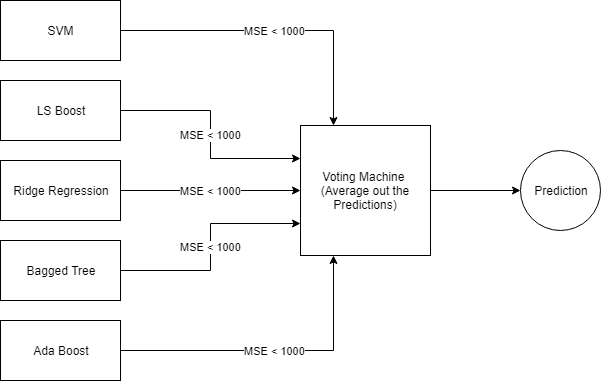
\includegraphics[width = 0.4\textwidth]{voting_model.png}
\label{vm}
\caption{This Fig. shows the voting model used in this experiment. The model will average the results of the models with MSE < 1000.}
\end{figure}

\subsection{Designing the Experiment}
Once the model has been designed, the next step is to build the experiment. Using the data set from Yahoo Financial Tool[10] and Kaggle[9], the Dow Jones Industrial Average companies were selected. These data were then separated into 2 data sets, training and testing. Although each company entered the stock market differently, the model will train all the historical data set up to November 2018. The testing set will be the data in November 2018. With weekends and the holiday, this experiment will have 21 different predictions. The reason why this experiment will train all the historical data before November 2018, instead of the general training 70\% of the data and test 30\% of the data is because this is experiment is used for future predictions. 

\begin{table}[H]
 \centering
 \caption{Number of training and testing data} 
\begin{tabularx}{0.5\textwidth}{| X | X | X |}

\hline
 & \textbf{train} &	\textbf{test}  \\ \hline
aapl & 9555 & 21   \\ \hline
axp & 11709 & 21  \\ \hline
ba & 14308 & 21  \\ \hline
cat	&14308 & 21 \\ \hline
csco& 	7234&	21	\\ \hline
cvx&	12321	&21	\\ \hline
dwdp&	11709&	21\\ \hline	
gs	&4908	&21\\ \hline
hd	&9360	&21\\ \hline
ibm	&14308&	21	\\ \hline
intc	&9743&	21\\ \hline
jnj	&12321	&21\\ \hline
jpm	&9743&	21\\ \hline
ko	&14308&	21\\ \hline
mcd	&12321&	21\\ \hline
mmm	&12321&	21\\ \hline
mrk	&12321&	21\\ \hline
msft	&8229&	21\\ \hline
nke	&9563	&21\\ \hline
pfe	&11709&	21\\ \hline
pg	&12321&	21\\ \hline
trv	&9743&	21\\ \hline
unh	&8582&	21\\ \hline
utx	&12321&	21\\ \hline
v	&2676&	21	\\ \hline
vz	&8811&	21\\ \hline
wba	&9743&	21\\ \hline
wmt	&11649&	21\\ \hline
xom	&14308&	21\\ \hline



\end{tabularx}
\label{Pinouts}
\end{table}

After these data sets are separated, it is worth analyzing these data. The data sets contain historical data. The historical data consists of the date of the trade. The day's high, low, opening, closing and volumes. The number of volumes was not used in this experiment. The other features, high, low, opening, and closing were relevant in this experiment. When it comes to stock market prediction, the goal is to predict the value of a stock. The question now, is what kind of price the model want to predict. In today's standards, where big corporations are using neural networks and other complex models, the stock prediction is predicting the price at a given time. These corporations are also given data sets where the prices are given within the seconds. Since the data set used in this experiment is not in seconds, but are in days, it would be reasonable to predict in days. Predicting the day's stock price is also tricky because a day's stock value can be seen as its high or low. In modern media the stock's high value is emphasized, to give confidence to the company and the investors. For this experiment, the closing was choosing. The closing was chosen to be the stock prediction because of multiple reasons. Sometimes companies announce a new product, the stocks would go up, but the closing will indicate how well the stock performed during the day. Sometimes, the stock price of a company decreases because of a recession, the closing helps save the companies from losing value. Though the prices will fall after hours, companies usually would try saving itself before investors starts selling their shares. \\

When the desired data was found the data was split up using Python. Python can simply read through CSV files and reorganize data. For this experiment, the dates were removed, and the number of volumes were also removed. The file was then split into 2 where one file had training data points and the other had testing training points. After that the next thing to do was to build the model. This experiment used MATLAB 2018a. MATLAB is a wonderful software to use for machine learning models. There are even built-in functions for some of these models. SVM machines unfortunately is no longer available in MATLAB. However, there are open source C code that can be used to generate a model for an SVM. Ridge regression is a built-in model in MATLAB. The 2 boosts in this experiment, LS Boost and Ada Boost are also available in MATLAB. Bagged Trees is also available in MATLAB. Each model will take in the training data set and generate a prediction set. The prediction set will then be checked by MATLAB's built-in mean square error calculation to check for accuracy. The voting model will then give a vote of the models with reasonable accuracy. 

%%%%%%%%%%% Results
\section{Results}
\subsection*{Experiment Results}
After the model was build, the experiment performed, and the data was recorded. Table II shows the results of the experiment. The Dow Jones company was recorded with the model's mean square error. The voting model was then recorded as well as the percent error.

\begin{table}[H]
 \centering
 \caption{Results from Doing the Voting Model on DowJones} 
\begin{tabularx}{0.5\textwidth}{| X | X | X | X | X | X | X | X |}

\hline
 &\textbf{svm mse} & \textbf{ridge mse} & \textbf{ls mse} & \textbf{bt mse} & \textbf{ada mse} & \textbf{model mse}	& \textbf{model \% error} \\ \hline
aapl & 5239.81 & 4.7911 & 7.3848 & 5.575 & 36134.6 & 5.1147 & 1.0133 \\ \hline
axp & 1011.56 & 0.80833 & 1.2217 & 1.5121 & 10042.8 & 1.0957	& 0.74304 \\ \hline
ba & 46449.4 & 23.4131 & 19.9025 & 25.583 & 103141 & 20.8903 & 1.1311 \\ \hline
cat	& 1579.12 & 3.1983 & 9.5451 & 3.5991 & 14264.4 & 3.38966 & 1.12658 \\ \hline
csco & 0.61826 & 0.1619 & 0.19295 & 0.20736 & 515.533 & 0.19325 & 0.75345 \\ \hline
cvx & 2.1963 & 1.3118 & 1.2696 & 1.2131 & 9966.36 & 1.2248 & 0.76479 \\ \hline
dis & 0.6439 & 0.43951 & 0.46463 & 0.45318 & 10319.6 & 0.37096 & 0.43647 \\ \hline
dwdp & 50.228 & 0.18355 & 0.48116 & 0.20738 & 1512.10 & 3.3446 & 1.13131 \\ \hline
gs & 3218 & 6.1805 & 5.3311 & 6.4343 & 8284.76 & 5.7827 & 0.74767 \\ \hline
hd & 1988.36 & 3.8388 & 4.0139 & 4.2216 & 31646.1 & 3.6708 & 0.94764 \\ \hline
ibm & 0.71935 & 1.0289 & 0.70922 & 0.71885 & 7929.05 & 0.65653 & 0.56535 \\ \hline
intc & 0.456 & 0.25909 & 0.42047 & 0.31059 & 2150.10 & 0.31067 & 0.98188 \\ \hline
jnj & 1305.94 & 1.0317 & 0.9956 & 1.1869 & 17780.1 & 0.95638 & 0.48624 \\ \hline
jpm & 0.8052 & 0.71791 & 0.43832 & 0.57102 & 5719.32 & 0.5152 & 0.54046 \\ \hline
ko & 264.356 & 0.11768 & 2.891 & 3.2433 & 1519.30 & 1.4674 & 2.2253 \\ \hline
mcd & 435.153 & 1.3684	& 56.997 & 62.1388 & 25676.5 & 27.748 & 2.6444 \\ \hline
mmm & 33050.2 & 4.1397 & 4.0157 & 3.4883 & 30056.1 & 3.7331 & 0.7624 \\ \hline
mrk & 0.33473 & 0.32593 & 0.28707 & 0.26173 & 3355.34 & 0.22958 & 0.5186 \\ \hline
msft & 500.922 & 1.1211 & 0.83372 & 0.86626 & 6115.66 & 0.83826 & 0.70753 \\ \hline
nke & 0.53578 & 0.47407 & 0.49285 & 0.38082 & 554.990 & 0.30938 & 0.60154 \\ \hline
pfe & 0.41078 & 0.12467 & 0.06741 & 0.06410 & 1844.04 & 0.10893 & 0.63337 \\ \hline
pg & 1.067 & 0.25772 & 0.3253 & 0.31612 & 6405.93 & 9.39894 & 0.53366 \\ \hline
trv	& 624.960 & 1.7258 & 1.1017 & 1.6286 & 12164.9 & 1.4375 & 0.74581 \\ \hline
unh & 20411.2 & 5.9988 & 25.9641 & 32.6517 & 69364.9 & 16.3455 & 1.1447 \\ \hline
utx	& 1.9193 & 1.0524 & 0.91133 & 0.77739 & 14802.3 & 0.80217 & 0.57549 \\ \hline
v & 10.2753 & 2.3743 & 0.99417 & 1.8449 & 3238.51 & 2.1772 & 0.74316 \\ \hline
vz & 0.66769 & 0.14876 & 0.16232 & 0.1509 & 909.055 & 0.16903 & 0.55395 \\ \hline
wba & 0.56608 & 0.32132 & 0.2442 & 0.25947 & 2899.22 & 0.25159 & 0.52558 \\ \hline
wmt & 333.775 & 0.50535 & 0.35499 & 0.49133 & 7707.03 & 0.36225 & 0.46993 \\ \hline
xom & 0.72208 & 0.48935 & 0.28839 & 0.32346 & 4629.73 & 0.30322 & 0.58332 \\ \hline



\end{tabularx}
\label{Pinouts}
\end{table}
Although Table II shows the models ran well. Pictorial presentations show a different results. Fig. 2 and Fig. 3 shows models that performed well.

\begin{figure}[H]
\centering
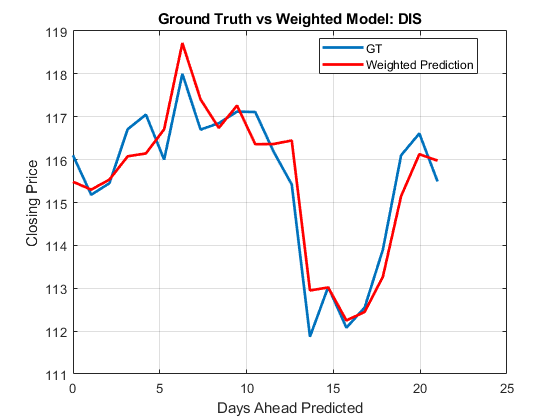
\includegraphics[width = 0.3\textwidth]{dis.png}
\label{dis}
\caption{This graph shows voting model prediction for Disney.}
\end{figure}

\begin{figure}[H]
\centering
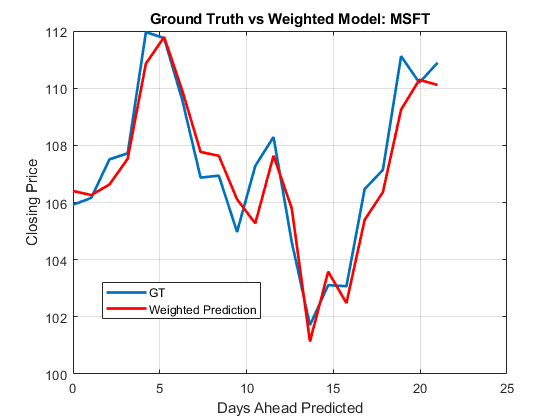
\includegraphics[width = 0.3\textwidth]{msft.png}
\label{msft}
\caption{This graph shows voting model prediction for Microsoft.}
\end{figure}

Fig. 4 and Fig. 5 shows 2 models that did not performed well.

\begin{figure}[H]
\centering
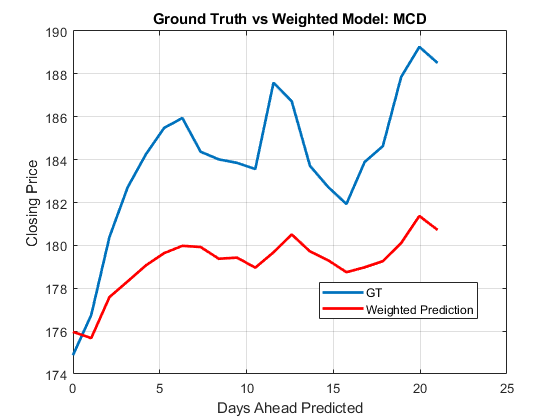
\includegraphics[width = 0.3\textwidth]{mcd.png}
\label{dis}
\caption{This graph shows voting model prediction for McDonald's.}
\end{figure}

\begin{figure}[H]
\centering
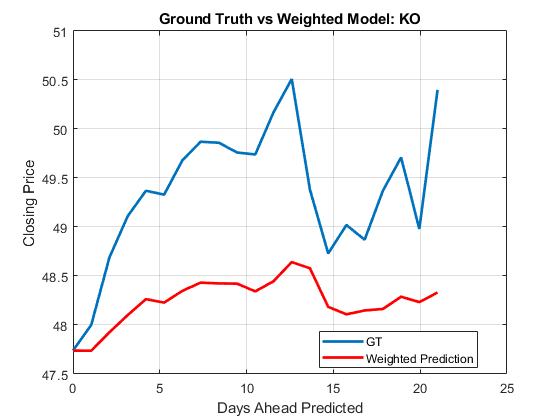
\includegraphics[width = 0.3\textwidth]{ko.png}
\label{msft}
\caption{This graph shows voting model prediction for Coca Cola.}
\end{figure}

\subsection*{Analysis}
Stock market prediction is a difficult experiment to perform. For this experiment there are many factors that can influence the results. For example, this model is predicting closing prices given a company's opening, highs and lows. When applying this to the real world, this is impossible. It is impossible to know a company's opening before the opening. The test assumes that that opening was known and was used in the model. Another impossible thing in the experiment was knowing the day's highs and lows. If this model were to be used to predict the value of stocks, this experiment will fail. Another thing that made this experiment unlikely to happen is the way the model predicted the future stock prices. In an actual scenario, the model will train everything into a model. The model will then be used to predict tomorrow's stock prices. After that, the prediction will be tested in its accuracy and the ground truth will be added to the prediction model. When the ground truth is added to the prediction model, the model would need to be retrained. After that the second day would be predicted and this cycle will happen again. The flaw in this experiment was training the model once and using that model to predict a month in advance. If the known openings, highs, and lows were not given, the models would have all given inaccurate predictions.\\

One thing that can be seen from all the models is that Ada Boost were giving high mean squared errors. This means that Ada Boost did not perform well in this experiment. It seems that Yang's[1] experiment only worked for the Shanghai markets. Ada Boost will not work for the Dow Jones. The experiment did however validate Sharma's[8] experiment. LS Boost and random forest provided accurate predictions. Both models also performed better than the SVM models. Adding the SVM model into the voting model may have made the prediction model predict inaccurate results. \\

Although most of the experiments did not use all 5 models in its prediction, some experiments did. An example of that is with Nike. Fig 6 shows the prediction of Nike. From analyzing the prediction results, when all 5 models are used in the voting model, it predicted better when comparing to each model individually. The goal to have the prediction model to do better than an SVM model is accomplished. 

\begin{figure}[H]
\centering
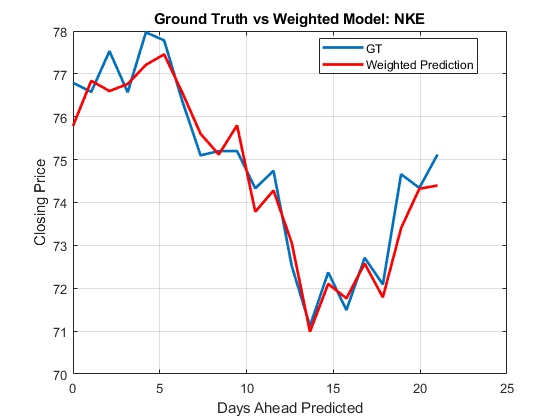
\includegraphics[width = 0.3\textwidth]{nke.png}
\label{nike}
\caption{This graph shows voting model prediction for Nike.}
\end{figure}

%%%%%%%%%%% Conclusion
\section{Conclusion}
In conclusion it can be seen that predicting the stock market is difficult. As an impossible task, there can be an accurate model. The stock market is not controlled by numbers, it is controlled by the public. If a company or establishment is providing services or products that benefits everyone, then investors will invest. From this experiment, this model will run well in theory of there is no sudden recession. The models will train itself well and predict a trend. There are many missing data when trying to predict the stock market. A perfect example is using a data set with politics. Politics is a heavy influence on the stock market. Companies are always regulated, and companies would always try to influence the government to better itself. It would be ideal for companies to have lobbyist in the government to advocate for more profits. However, a data set of this would backfire the companies. However, lobbyists do exist and companies use them to influence the government to maximize its value. Another data set that would be useful to predict stock market is public opinion. Companies, especially the Dow Jones requires positive public opinion. Having a data set of people's opinions in social media is useful to have. Most of the models in this experiment did not allow all 5 models to vote, and some models had only 3 votes. A neural network might be a better model to use. It would be quicker and using the suggested datasets could make the predictions better.

%%%%%%%%%%% Regerences
\begin{thebibliography}{}
\bibitem{ref 1}H. Yang, X. Liu and Q. Wu, "A Practical Machine Learning Approach for Dynamic Stock Recommendation," 2018 17th IEEE International Conference On Trust, Security And Privacy In Computing And Communications/ 12th IEEE International Conference On Big Data Science And Engineering (TrustCom/BigDataSE), New York, NY, 2018, pp. 1693-1697
\bibitem{ref 2} J. Yang, R. Rao, P. Hong and P. Ding, "Ensemble Model for Stock Price Movement Trend Prediction on Different Investing Periods," 2016 12th International Conference on Computational Intelligence and Security (CIS), Wuxi, 2016, pp. 358-361.
\bibitem{ref 3}R. Y. Nivetha and C. Dhaya, "Developing a Prediction Model for Stock Analysis," 2017 International Conference on Technical Advancements in Computers and Communications (ICTACC), Melmaurvathur, 2017, pp. 1-3.
\bibitem{ref 4}I. Kumar, K. Dogra, C. Utreja and P. Yadav, "A Comparative Study of Supervised Machine Learning Algorithms for Stock Market Trend Prediction," 2018 Second International Conference on Inventive Communication and Computational Technologies (ICICCT), Coimbatore, 2018, pp. 1003-1007.
\bibitem{ref 5} M. Usmani, S. H. Adil, K. Raza and S. S. A. Ali, "Stock market prediction using machine learning techniques," 2016 3rd International Conference on Computer and Information Sciences (ICCOINS), Kuala Lumpur, 2016, pp. 322-327.
\bibitem{ref 6}S. Das, "A volatility-driven stock trading framework based on automated, short-term recommendation method," 2017 IEEE 7th Annual Computing and Communication Workshop and Conference (CCWC), Las Vegas, NV, 2017, pp. 1-6.
\bibitem{ref 7}R. T. Gonzalez, C. A. Padilha and D. A. C. Barone, "Ensemble system based on genetic algorithm for stock market forecasting," 2015 IEEE Congress on Evolutionary Computation (CEC), Sendai, 2015, pp. 3102-3108.
\bibitem{ref 8}N. Sharma and A. Juneja, "Combining of random forest estimates using LSboost for stock market index prediction," 2017 2nd International Conference for Convergence in Technology (I2CT), Mumbai, 2017, pp. 1199-1202.
\bibitem{ref 9}B. Marjanovic, "Huge Stock Market Dataset", Kaggle.com, 2017. [Online]. Available: \url{https://www.kaggle.com/borismarjanovic/price-volume-data-for-all-us-stocks-etfs}. [Accessed: 27- Nov- 2018]
\bibitem{ref10}“Stock Screener,” Yahoo! Finance. [Online]. Available: https://finance.yahoo.com/screener/. [Accessed: 15-Dec-2018].
\end{thebibliography}

%%%%%%%%%%% Biography
%\begin{IEEEbiography}[{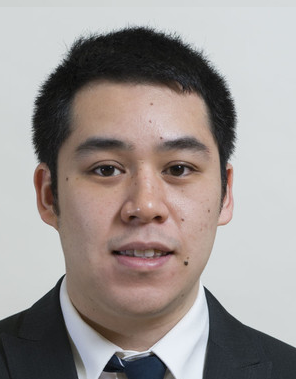
\includegraphics[width=1in,height=1.25in,clip,keepaspectratio]{wu_barry_professional_photo.png}}]{Barry Wu}
\begin{IEEEbiographynophoto}{Barry Wu}
is a 5$^{th}$ year computer engineering student in Rochester Institute of Technology. He is fascinated by the how dynamic the stock market and is interested in building a robust predictive model. His interest in the stock market was influenced from growing up in New York City and meeting many successful businessmen and businesswomen. He chose the path of engineering as the technology industry shows promising future in building a stock portfolio. Aside from engineering, Barry is interested in origami.
%\end{IEEEbiography}
\end{IEEEbiographynophoto}

\section{Appendix}
This section contains the Appendix. This section shows the graphical presentation of the models with each model and the weighted model. 

%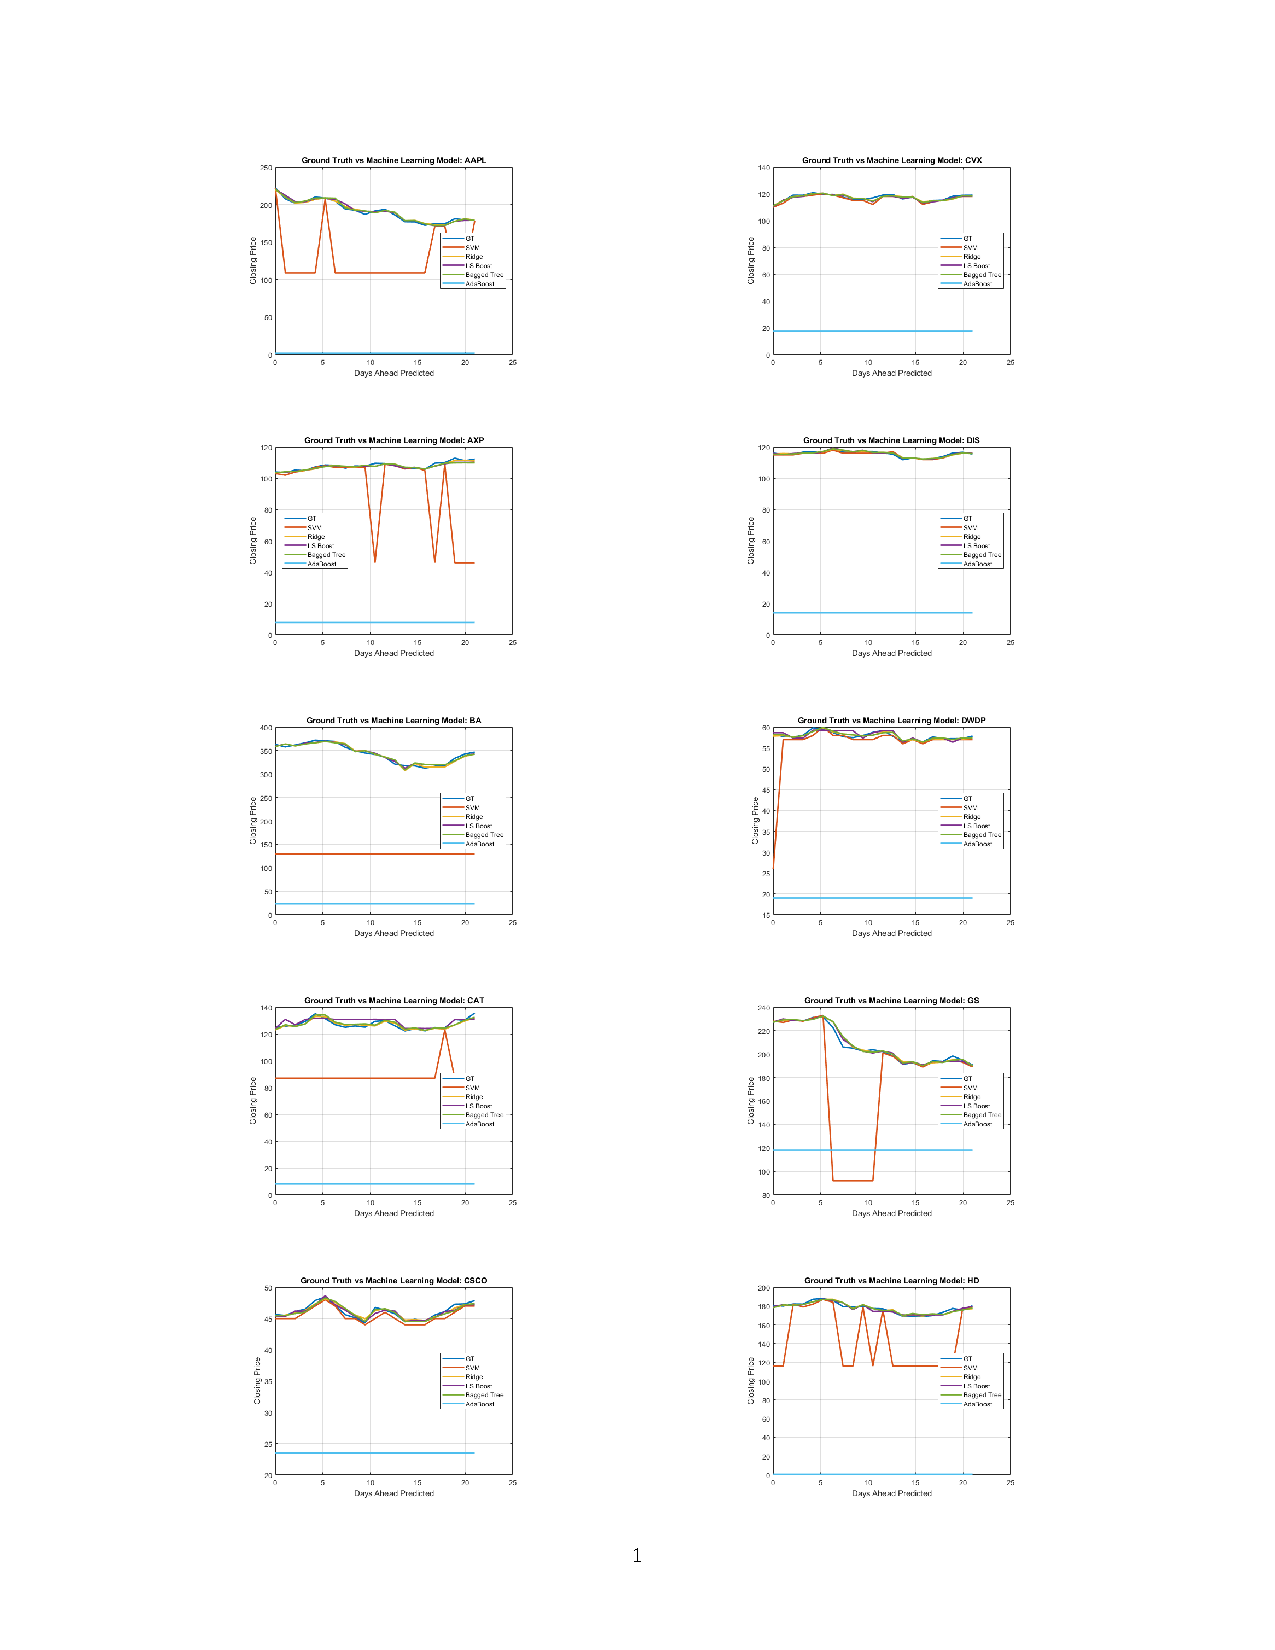
\includepdf[pages=-]{training.pdf}
%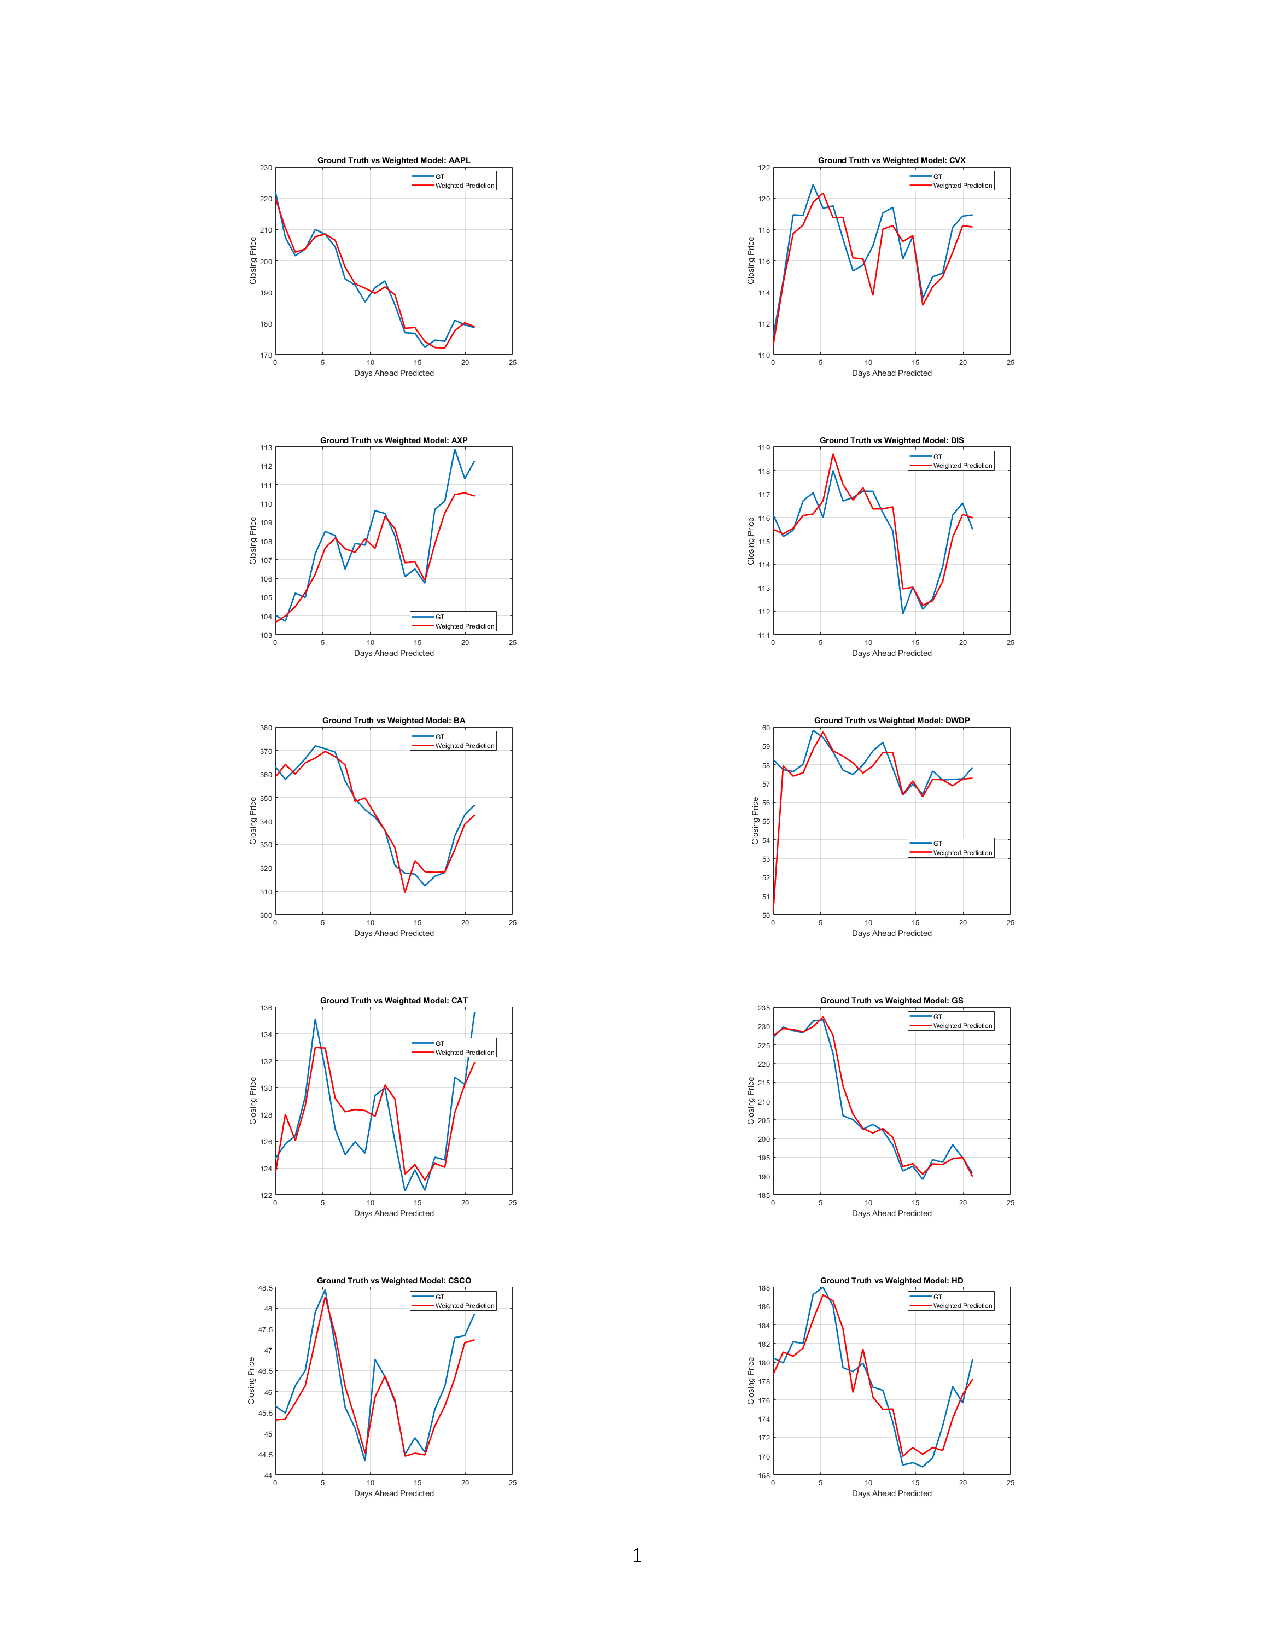
\includepdf[pages=-]{testing.pdf}
\end{document}
